%
%
%
%
%
\chapter{Aerodynamic Forcing Functions}
\label{waves.chap}
\headc{Aerodynamic forcing functions}
\setcounter{footnote}{0}
%
 A method for calculating potential, vortical and entropic
 components of unsteady flow-field is presented in this appendix.
 The method, based upon the Goldstein's splitting theorem and the linearised
 acoustic equations, evaluates the aerodynamic forcing functions
 from a steady-state solution to impose as on coming unsteadiness to a single bladerow.
 Such boundary conditions can be used for both linear and non-linear unsteady
 computations with the difference that, for the linear simulation,
 only one harmonic at a time can be used.
 The procedure starts from some steady-state data of the adjacent bladerow
 boundary, either the outflow of the upstream blade or the inflow of the
 downstream blade. The steady-state flow data could be either computed or measured.
%
%
%
%
\section{Spatial Non-uniformities}
%
 The first step for calculating the aerodynamic forcing functions,
 originating from an adjacent bladerow, is to analyse
 the Fourier components of the data at a given far-field boundary.
 In the reference frame fixed with a given blade row `1',
 the flow field is steady but possesses spatial flow non-uniformities.
 In this way, at a given far-field boundary
 the steady-state primitive variables, in axisymmetric coordinates,
 can be expressed as the sum of an axisymmetric steady-state part plus
 a steady-state non-uniform part:

%
\beq
  {\bf V}\left(x,\theta\sm{1},r\right) = \overline{\bf V}\left(x,r\right) +
                                         \widetilde{\bf V}\left(x,\theta\sm{1},r\right)
\eeq
%
 The steady-state non-uniform part can be Fourier decomposed because
 of periodicity in the tangential direction.

%
\beq
  \widetilde{\bf V}\left(x,\theta\sm{1},r\right) =
  \sum \widetilde{\bf V}\sm{m}\left(x,r\right)
  \exp{\left(i\kappa\sm{\theta}\theta\sm{1}\right)}
  \label{perurbation_variables.eq}
\eeq
%
 The tangential wave number $\kappa\sm{\theta}$ is given by

%
\beq
  \kappa\sm{\theta} = \frac{2\pi m}{\Delta \theta\sm{1}}
  \label{tangential_wave_number.eq}
\eeq
%
 where $\Delta \theta\sm{1}$ is the blade-to-blade spacing
 and $m$ is the mode number.

 If one considers a bladerow `2', adjacent to bladerow `1', then
 the tangential positions $\theta\sm{1}$ and $\theta\sm{2}$ are
 related to the rotational velocities $\Omega\sm{1}$ and $\Omega\sm{2}$
 and time $t$ by:

%
\beq
 \theta\sm{1} + \Omega\sm{1}t = \theta\sm{2} + \Omega\sm{2}t
  \label{rota12.eq}
\eeq
%
 Substituting (\ref{rota12.eq}) into (\ref{tangential_wave_number.eq})
 one can obtain:

%
\beq
  \frac{2\pi m}{\Delta \theta\sm{1}}\theta\sm{1} =
  \frac{2\pi m}{\Delta \theta\sm{1}}\theta\sm{2} -
  \frac{2\pi m\left(\Omega\sm{1}-\Omega\sm{2}\right)}{\Delta \theta\sm{1}}t
\eeq
%
 and in a different notation;

%
\beq
  \frac{2\pi m}{\Delta \theta\sm{1}}\theta\sm{1} =
  -\frac{\phi\sm{2}}{\Delta \theta\sm{2}}\theta\sm{2} - \omega\sm{2} t
\eeq
%
 So the the stationary $m\se{th}$ mode in bladerow `1' is equivalent to an unsteady
 mode in blade row `2' with reduced frequency

%
\beq
  \omega\sm{2} = \frac{2\pi m\left(\Omega\sm{1}-\Omega\sm{2}\right)}{\Delta \theta\sm{1}}
  \label{frequency_rotaz.eq}
\eeq
%
 and interblade phase angle:

%
\beq
  \phi\sm{2} = -\frac{2\pi m \Delta \theta\sm{2}}{\Delta \theta\sm{1}}
  \label{nterblade_phase_angle.eq}
\eeq
%
 In order to maintain all frequencies $\omega\sm{2}$ positive, the summation in
 (\ref{perurbation_variables.eq}) has to be for $m > 0$ in the case of
 $\left(\Omega\sm{1} - \Omega\sm{2}\right) > 0$ and for $m < 0$ in the case of
 $\left(\Omega\sm{1} - \Omega\sm{2}\right) < 0$.

 The harmonic boundary terms that go with this mode are:

%
\beq
  \widehat{\bf V}\left(x,\theta\sm{2},r\right) =
  \widetilde{\bf V}\sm{m}\left(x,r\right)
  \exp{\left(-\frac{i\phi\sm{2}}{\Delta \theta\sm{2}}\theta\sm{2}\right)}
\eeq
%
%
%
%
\section{Vortical, Potential and Entropy Splitting}
\headc{Aerodynamic forcing functions}
%
 In the development of the linear theory, the flow non-uniformities
 $\widetilde{\bf V}\left(x,\theta,r\right)$ are assumed to be small
 relative to the uniform steady flow properties $\overline{\bf V}\left(x,r\right)$.
 Under such approximation it is possible to recover the linearised acoustic
 equations (Anderson \citeyearNP{Anderson:2}).

%
\beq
  \frac{1}{\overline{c}\se{2}} \ftot{\widetilde{p}} +
  \overline{\rho}\ \nabl\cdot\widetilde{\vec{v}} &=& 0
  \label{acoustic_equation_1.eq}\\
  \overline{\rho} \ftot{\widetilde{\vec{v}}} +
  \nabl\widetilde{p} &=& 0
  \label{acoustic_equation_2.eq}\\
  \ftot{\widetilde{s}} = 0
  \label{acoustic_equation_3.eq}
\eeq
%
 According to Goldstein's splitting theorem (Goldstein \citeyearNP{Goldstein:1}),
 the perturbation velocity $\widetilde{\vec{v}}$ can be decomposed into the sum
 of (i) a rotational component $\widetilde{\vec{v}}\sm{v}$ that is purely convected,
 has zero divergence and is
 completely decoupled from the fluctuations in pressure or in any other thermodynamic
 property and (ii) an irrotational disturbance $\widetilde{\vec{v}}\sm{p}$ that
 produces no entropy fluctuations
 but is directly related to the pressure fluctuations.

%
\beq
   \widetilde{\vec{v}} = \widetilde{\vec{v}}\sm{v} + \widetilde{\vec{v}}\sm{p}
   \label{Goldstein_splitting.eq}
\eeq
%
 The rotational velocity field is also known as the vortical perturbation, and
 the irrotational perturbation is also referred to as the potential (or
 acoustic) perturbation.
 Finally the fluctuations in entropy are decoupled from the velocity and pressure
 fluctuations, but do produce density fluctuations which are convected with the flow.

 Summarizing, three different modes of motion can be solution of the linearised
 acoustic equations (\ref{acoustic_equation_1.eq}-\ref{acoustic_equation_3.eq}):
 vortical, potential and entropy mode.
 In the following three paragraphs these modes will be analysed in detail
 in axisymmetric coordinate, neglecting the radial components of $\vec{v}$.
%
%
\subsubsection{Vortical mode}
%
 The Goldstein's splitting assumes that any vortical perturbation satisfies
 the following constraints:

%
\beq
  \nabl\cdot\widetilde{\vec{v}}\sm{v} &=& 0
  \label{vortical_1.eq}\\
  \ftot{\widetilde{\vec{v}}\sm{v}} &=& 0
  \label{vortical_2.eq}\\
  \widetilde{p}\sm{v} &=& 0
  \label{vortical_3.eq}\\
  \widetilde{\rho}\sm{v} &=& 0
  \label{vortical_4.eq}
\eeq
%
 The steady-state form of (\ref{vortical_2.eq}) shows that the vortical propagation
 wave vector $\vec{\kappa}$ must be perpendicular to the blade mean flow exit
 velocity vector.
 Hence the scalar product must be zero:

%
\beq
  \vec{k}\cdot\overline{\vec{v}} = 0
  \label{vortical_5.eq}
\eeq
%
 The tangential wave number is given in (\ref{tangential_wave_number.eq}) while the
 axial wave number of the vortical mode, derived from
 (\ref{vortical_5.eq}) becomes:

%
\beq
  \kappa\sm{x_m} = -\frac{\overline{v}\sm{\theta}}{\overline{v}\sm{x}}
                    \kappa\sm{\theta_m}
  \label{axial_wave_number.eq}
\eeq
%
 From (\ref{vortical_1.eq}) and (\ref{vortical_5.eq}), it is straightforward
 to show that the vortical mode magnitude vector must be parallel to the mean
 flow exit velocity vector. Denoting the complex constant of proportionality $D\sm{m}$
 the vortical perturbation can be written as:

%
\beq
  \widetilde{\vec{v}}\sm{v} = \overline{\vec{v}}\sum D\sm{m}
                            \exp\left(i\vec{\kappa}\sm{m}\cdot\vec{x}\right)
                            = \overline{\vec{v}}\sum D\sm{m}
                            \exp\left[i{\kappa}\sm{\theta_m}
       \left(\theta - \frac{\overline{v}\sm{\theta}}{\overline{v}\sm{x}}x\right)\right]
 \label{vortical_perturbation.eq}
\eeq
%
 Equation (\ref{vortical_perturbation.eq}) shows that the vortical
 perturbation propagates unattenuated both in the tangential and axial directions
 ($\vec{\kappa}$ contains only real part). Section \ref{Splitting.sec} will
 show how to calculate the complex constant of proportionality $D\sm{m}$.
%
%
%
\subsubsection{Potential mode}
%
 The potential velocity field can be derived from a potential function

%
\beq
  \widetilde{\vec{v}}\sm{p} = \nabl \psi\sm{p}
  \label{potential_1.eq}
\eeq
%
 and the perturbation potential is related to the perturbation pressure
 through the unsteady Bernoulli equation

%
\beq
  \widetilde{p}\sm{p} = -\overline{\rho}\ftot{\psi\sm{p}}
  \label{potential_2.eq}
\eeq
%
 The isentropic relation gives the perturbation density as a function of the
 perturbation pressure

%
\beq
  \widetilde{\rho}\sm{p} = \frac{1}{\overline{c}\se{2}}\widetilde{p}\sm{p}
  \label{potential_3.eq}
\eeq
%
 Combing equations (\ref{potential_1.eq}) and (\ref{potential_2.eq}) with
 (\ref{acoustic_equation_1.eq}) it is possible to obtain the following
 linear velocity potential equation.

%
\beq
  & &
  \frac{1}{c\se{2}}\psi\sm{p_{tt}}+
  \frac{2}{c}\left(\overline{M}\sm{x}\psi\sm{p_{xt}}+
                   \overline{M}\sm{\theta}\psi\sm{p_{\theta t}}\right) =
  \nonumber\\
  & &
  \left(1 - \overline{M}\sm{x}\se{2}\right) \psi\sm{p_{xx}} -
  2 \overline{M}\sm{x}\overline{M}\sm{\theta} \psi\sm{p_{x\theta}} +
  \left(1 - \overline{M}\sm{\theta}\se{2}\right) \psi\sm{p_{\theta\theta}}
  \label{potential_4.eq}
\eeq
%
 The steady-state version of (\ref{potential_4.eq}) has solutions of the form:

%
\beq
  \psi\sm{p} = \sum A\sm{m} \exp\left(i\kappa\sm{\theta_m}\theta + \chi\sm{m} x\right)
  \label{potential_5.eq}
\eeq
%
 where the axial decay $\chi\sm{m}$ is

%
\beq
  \chi\sm{m} = \frac{i\overline{M}\sm{x}\overline{M}\sm{\theta}
                     \pm {\rm sign}\left(\kappa\sm{\theta_m}\right)
                     \sqrt{1 - \overline{M}\se{2}}}{1-\overline{M}\sm{x}\se{2}}
                     \kappa\sm{\theta_m}
  \label{potential_6.eq}
\eeq
%
 Clearly the qualitative behaviour of this perturbation depends on whether the flow
 is subsonic or supersonic.

 ~\newline
 \underline{Subsonic mean flow} $\left(\overline{M} < 1\right)$: $\chi\sm{m}$ has both real and imaginary
 components. If one is interested in perturbation at the inlet boundary, then it is not
 physical to have perturbation growing exponentially downstream, and so the negative
 root of (\ref{potential_6.eq}) must be chosen.
 On the other hand, the positive root must be chosen
 for perturbation at outlet boundary.
 It is interesting to note that the rate of decay of the perturbation depends linearly
 on the tangential wave number component $\kappa\sm{\theta_m}$. As a consequence the most important
 mode is the fundamental mode $\kappa\sm{\theta_1} = \frac{2\pi}{\Delta \theta}$.

 ~\newline
 \underline{Supersonic mean flow} $\left(\overline{M} > 1\right)$: if the flow is
 still axially subsonic $\left(\overline{M}\sm{x} < 1\right)$, $\chi\sm{m}$ has only an
 imaginary component. To determine which root should be chosen in (\ref{potential_6.eq}),
 the supersonic characteristic theory has to be used (Giles \citeyearNP{Giles:4}).
 For an inlet boundary, the positive root should be chosen if the flow angle is positive and
 negative root if the flow angle is negative, vice-versa for an outlet boundary.
%
%
%
\subsubsection{Entropy mode}
%
 This mode is associated only with density fluctuations and like the
 vortical perturbation is convected with the mean flow, without any axial
 decay:

%
\beq
  \widetilde{\rho}\sm{e} &=& \overline{\rho}\sum B\sm{m}
       \exp\left[i\kappa\sm{\theta_m}\left(\theta -
       \frac{\overline{v}\sm{\theta}}{\overline{v}\sm{x}}x\right)\right]
  \label{entropy_perturbation.eq}\\
  \widetilde{\vec{v}}\sm{e} &=& 0\\
  \widetilde{p}\sm{e} &=& 0
\eeq
%
%
%
\section{Matching Linear Theory and Available Data}
\headc{Aerodynamic forcing functions}
\label{Splitting.sec}
%
 The complex constants $A\sm{m}$, $B\sm{m}$ and $D\sm{m}$ can be determined
 by matching  the linear theory with the measured or computed perturbation
 quantities $\widetilde{\bf V}$ (Manwaring \citeyearNP{Manwaring:1}).

 Using equations ({\ref{vortical_perturbation.eq}),(\ref{potential_1.eq}),
 (\ref{potential_2.eq}) and (\ref{potential_5.eq}) the relationship between the
 linear theory and the perturbation quantities $\widetilde{\bf V}$
 can be expressed as:

%
\beq
\left[
\begin{array}{cc}
 \chi\sm{m} & \overline{v}\sm{x}\\
 i\kappa\sm{m} & \overline{v}\sm{\theta}\\
-\overline{\rho}\left(\overline{v}\sm{x}\chi\sm{m}+
                  i\overline{v}\sm{\theta}\kappa\sm{m}\right) & 0
\end{array}
\right]
\left\{
\begin{array}{c}
A\sm{m}\\D\sm{m}
\end{array}
\right\}
=
\left[
\begin{array}{c}
\widetilde{v}\sm{x_m}\\
\widetilde{v}\sm{\theta_m}\\
\widetilde{p}\sm{m}\\
\end{array}
\right]
 \label{wave_deco_1.eq}
\eeq
%
 and combing (\ref{entropy_perturbation.eq}) and (\ref{potential_5.eq})

%
\beq
  B\sm{m} = \frac{1}{\overline{\rho}}\left(\widetilde{\rho}\sm{m} -
                            \frac{1}{c\se{2}}\widetilde{p}\sm{m}\right)
 \label{wave_deco_2.eq}
\eeq
%
 System (\ref{wave_deco_1.eq}) can also written in a compact notation

%
\beq
 \left[{\bf T}\right] {\bf a} = {\bf b}
 \label{wave_deco_3.eq}
\eeq
%
 Matrix $\left[{\bf T}\right]$ depends on the tangential wave number, thus $A\sm{m}$ and $D\sm{m}$
 take different values for each harmonic analysed.
 Relation (\ref{wave_deco_3.eq})  represents an overdetermined system of equations
 which can be solved using a least-squares (LS) method which minimizes the
 L2 norm of the difference between $\left[{\bf T}\right]{\bf a}$ and ${\bf b}$.
 The most widely used method for solving a full column rank
 \footnote{A Least squares problem
 $\left[{\bf T}\right] {\bf a} = {\bf b}$
 with $\left[{\bf T}\right] \in {\tt Re}\se{m\times n}$,
 ${\bf a} \in {\tt Re}\se{n}$ and ${\bf b} \in {\tt Re}\se{m}$
 is said to be full column rank
 when {\em rank}$\left[{\bf T}\right] = n$, i.e.
 the columns of $\left[{\bf T}\right]$ are linear
 independent.}
 LS problem  is the method of normal equations
 (Golub et al. \citeyearNP{Golub:1}).

 Introducing a diagonal weighting matrix $\left[{\bf W}\right]$ specifying
 the relative weighting of the three quantities on the right-hand side
 of (\ref{wave_deco_1.eq}), a LS solution of (\ref{wave_deco_3.eq}),
 using the method of normal equations, is given by:

%
\beq
 \left[{\bf T}\right]\se{T}\left[{\bf W}\right]\left[{\bf T}\right]{\bf a} &=&
 \left[{\bf T}\right]\se{T}\left[{\bf W}\right]{\bf b}
 \label{wave_deco_4.eq}
\eeq
%
 Following the procedure of Feiereisen et al. \citeyear{Feiereisen:1},
 only two weighting factors are used in ${\bf W}$: $W\sm{v}$ for the two velocity
 components $\widetilde{v}\sm{x_m}$, $\widetilde{v}\sm{\theta_m}$ and $W\sm{p}$ for the
 static pressure $\widetilde{p}\sm{m}$:

%
\beq
  \left[{\bf W}\right] = \left[
 \begin{array}{ccc}
 W\sm{v} & 0 & 0\\
 0 & W\sm{v} & 0\\
 0 & 0 & W\sm{p}\\
 \end{array}
\right]
\eeq
%
 The LS method will break down in two distinct cases: (i) $W\sm{v} = 0$ and
 (ii) incompressible flow with $W\sm{v} = W\sm{p}$
 (Feiereisen et al. \citeyearNP{Feiereisen:1}).
%
%
%
\section{Example}
%
\begin{figure}
 \begin{center}
  \begin{tabular}{cc}
    \subfigure[Velocity]
     {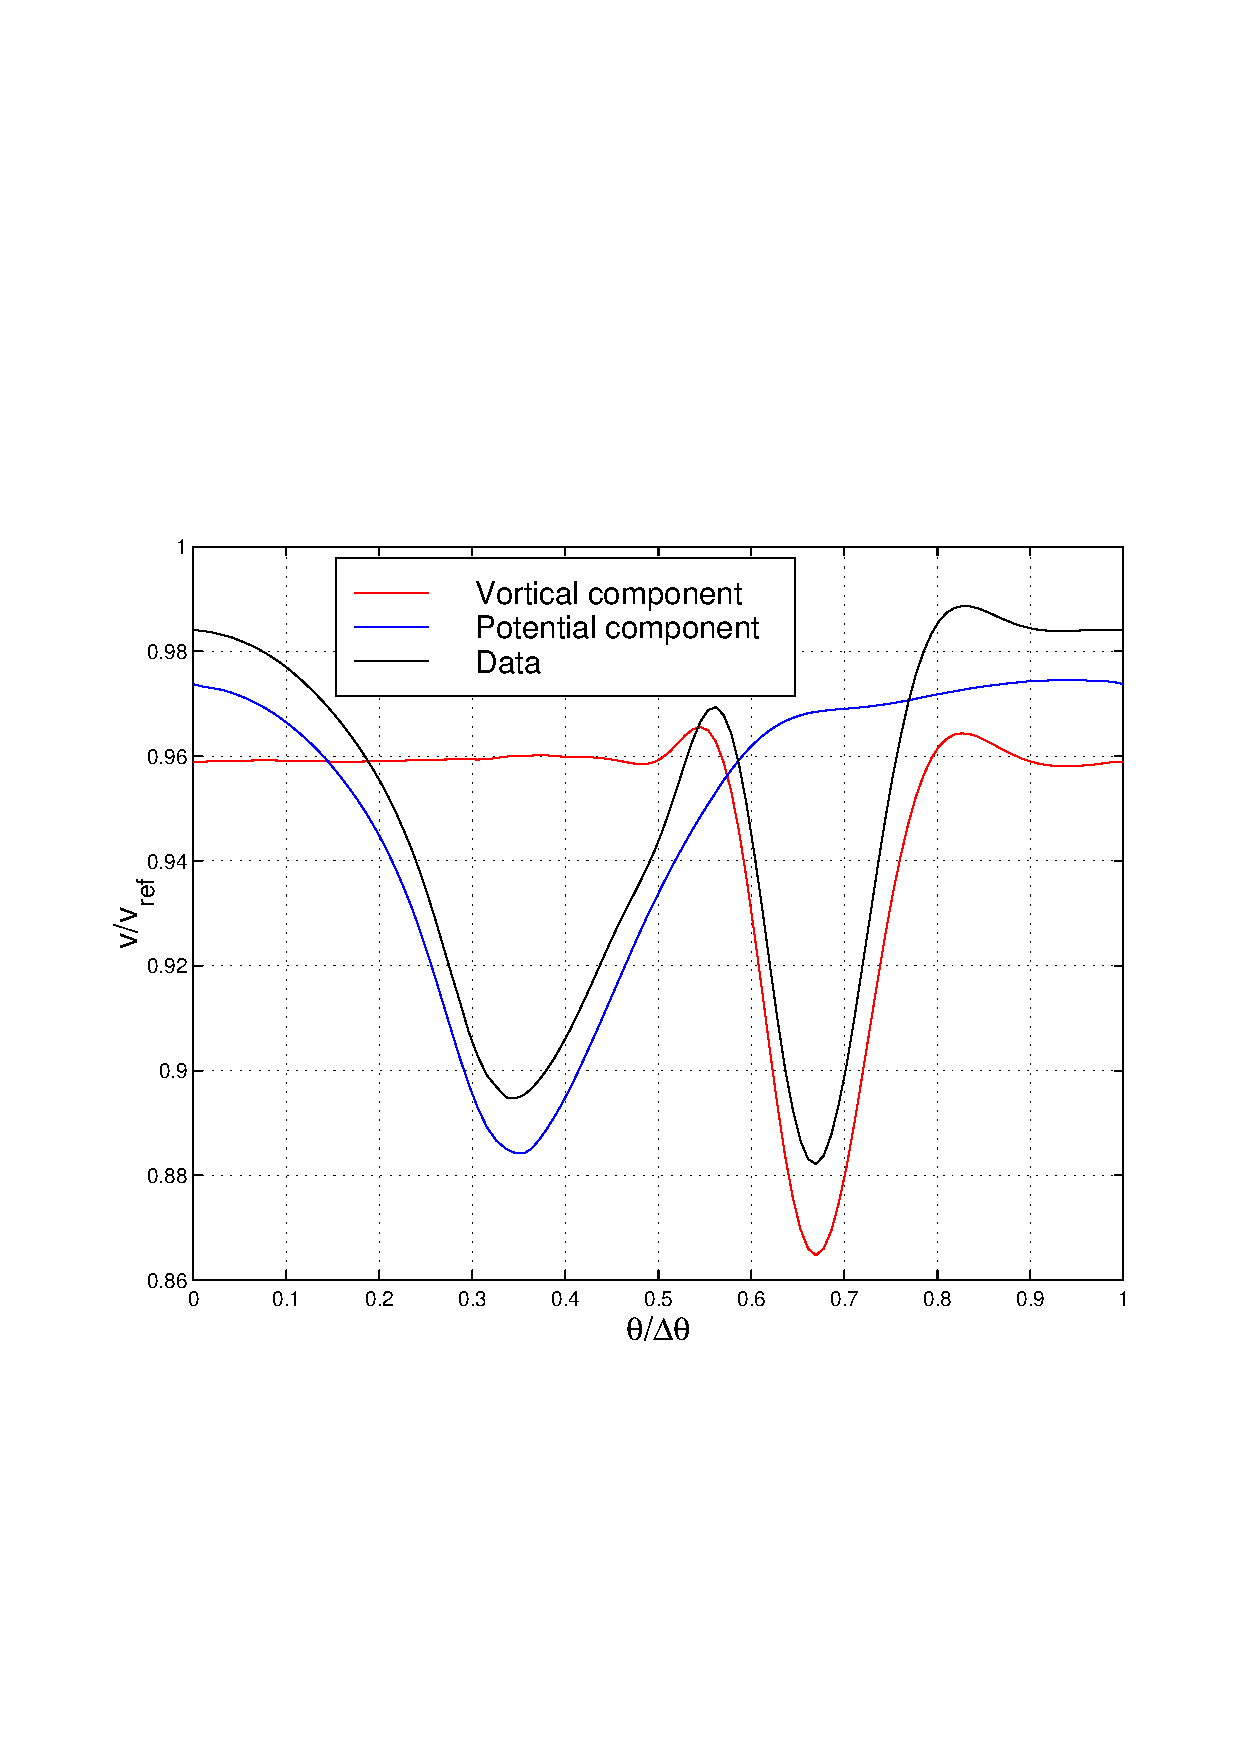
\includegraphics[height=55mm,clip=t]{APPEND/FIGURE/velo.pdf}}
        &
    \subfigure[Density]
     {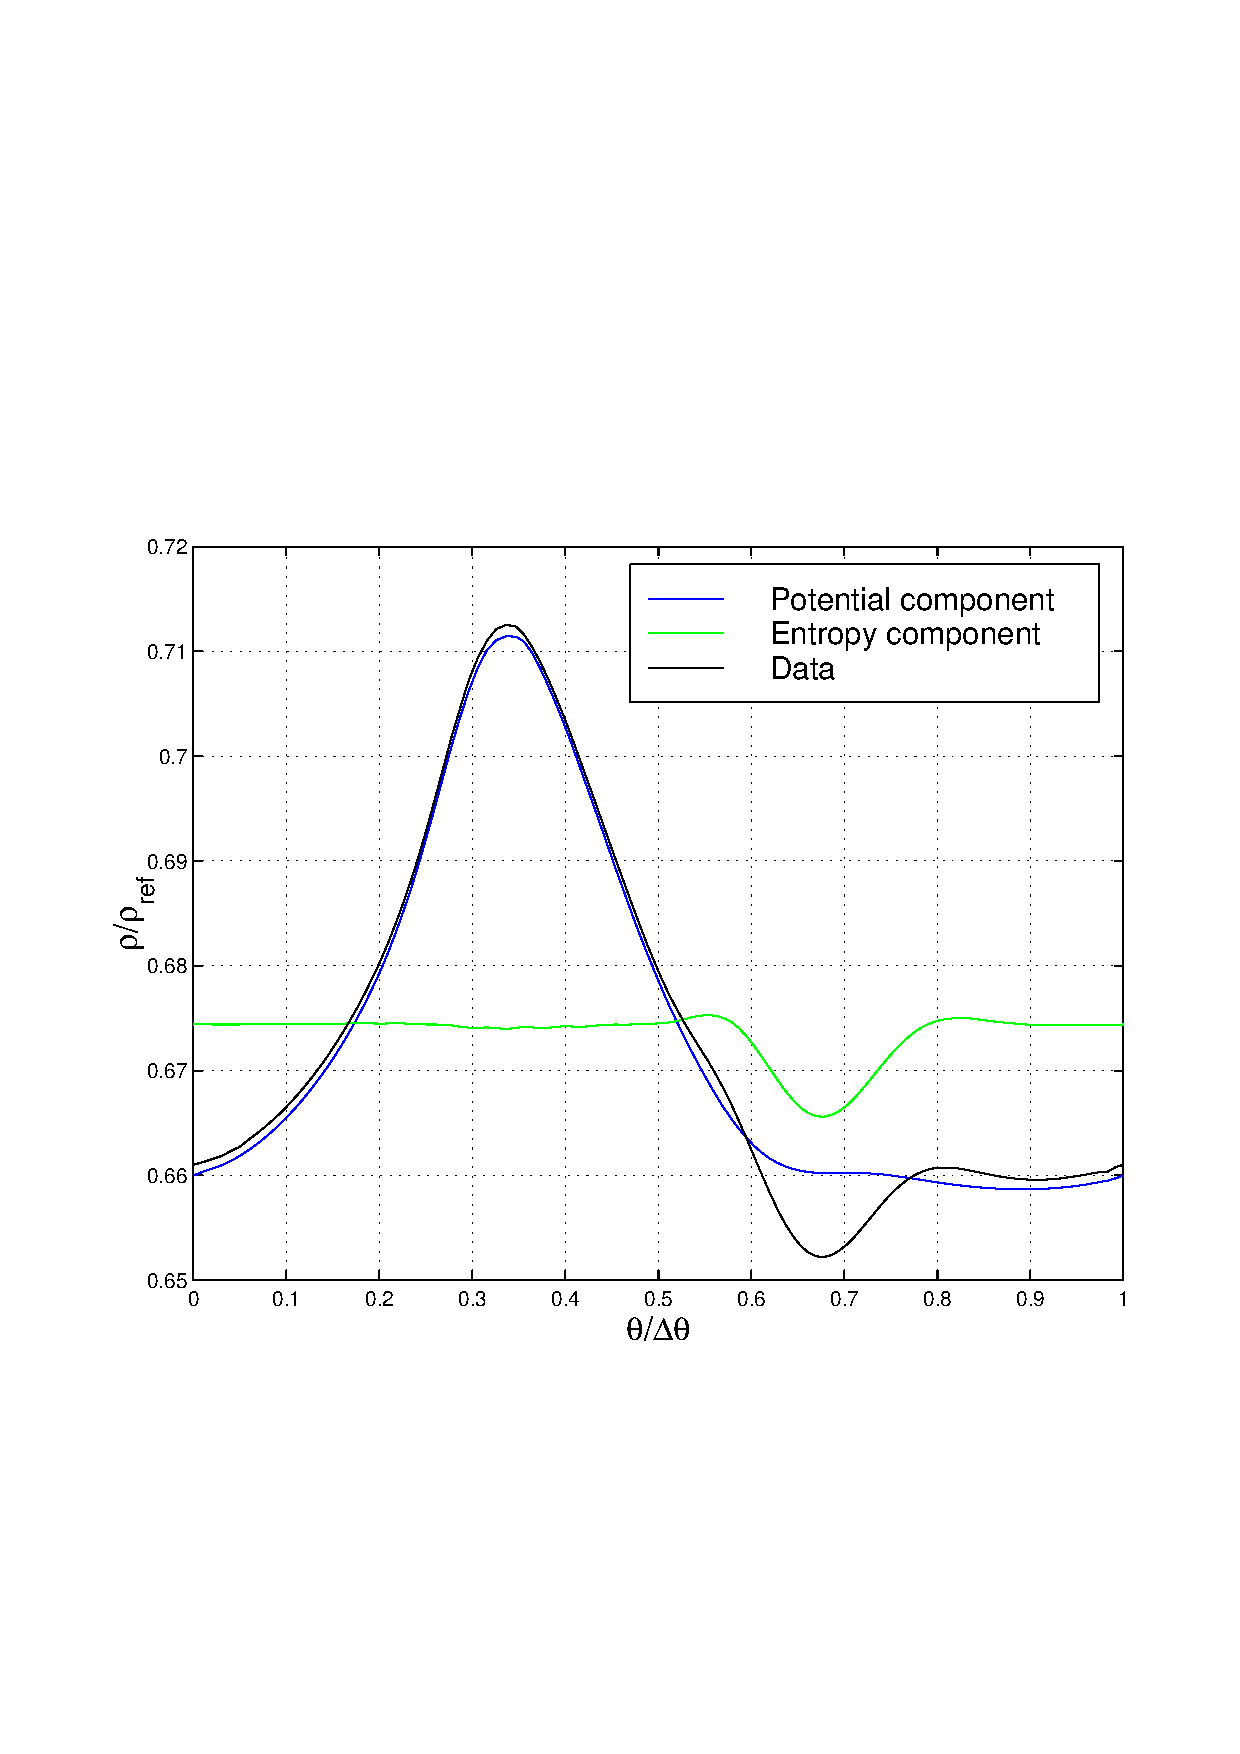
\includegraphics[height=55mm,clip=t]{APPEND/FIGURE/dens.pdf}}
        \vspace{-4mm}\\
    \subfigure[Pressure]
     {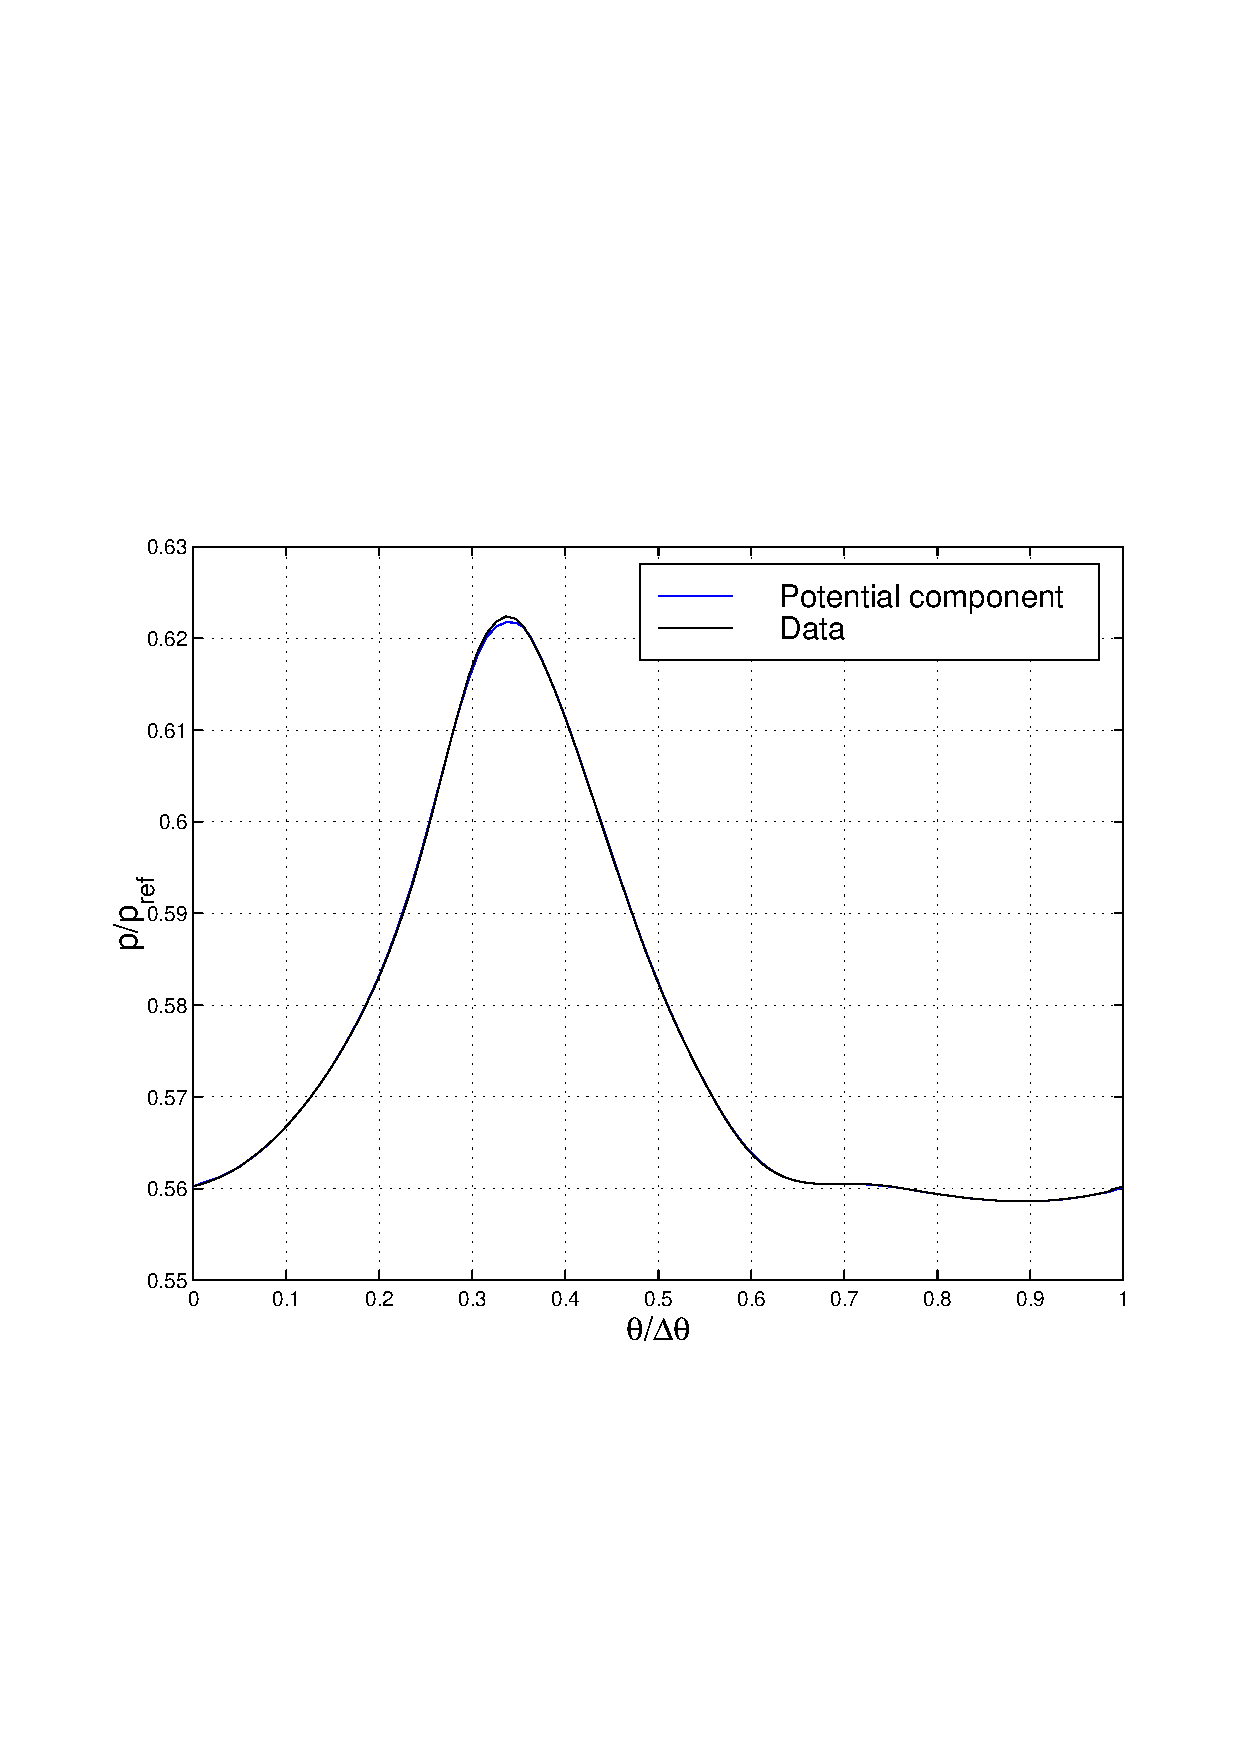
\includegraphics[height=55mm,clip=t]{APPEND/FIGURE/pres.pdf}}
        &
  \end{tabular}
 \end{center}
 \vspace{-5mm}
 \caption{Comparison between the computed steady data and the reconstructed
          vortical, potential and entropy components using first 10 harmonics.}
 \label{waves3.fig}
\end{figure}
%
 In order to illustrate the proposed method, let us consider the outflow
 boundary of a stator blade. The computed data is first Fourier decomposed
 along the tangential direction and then
 system (\ref{wave_deco_4.eq}) is solved for each Fourier component,
 to obtain the vortical, potential and entropy waves amplitudes $D\sm{m}$, $A\sm{m}$
 and $B\sm{m}$, using $W\sm{v}=W\sm{p}=0.5$.
 These quantities are then used to reconstruct the flow quantities
 at the boundary using an inverse Fourier transform.
 The results are shown in Fig. \ref{waves3.fig} where the reconstructed variables
 are obtained using the first Fourier components.
%
